%%%%%%%%%%%%%%%%%%%%%%%%%%%%%%%%%%%%%%%%%%%%%%%%%%%%%%%%%%%%%%%%%%%%%%%%%%%%%%%%%%%%%%%%%%%%%%%%%%%%%%%%%%%%%%%%%%%%%%%%%%%%%%%%%%%%%%%%%%%%%%%%%%%%%%%%%%%
% This is just an example/guide for you to refer to when submitting manuscripts to Frontiers, it is not mandatory to use Frontiers .cls files nor frontiers.tex  %
% This will only generate the Manuscript, the final article will be typeset by Frontiers after acceptance.   
%                                              %
%                                                                                                                                                         %
% When submitting your files, remember to upload this *tex file, the pdf generated with it, the *bib file (if bibliography is not within the *tex) and all the figures.
%%%%%%%%%%%%%%%%%%%%%%%%%%%%%%%%%%%%%%%%%%%%%%%%%%%%%%%%%%%%%%%%%%%%%%%%%%%%%%%%%%%%%%%%%%%%%%%%%%%%%%%%%%%%%%%%%%%%%%%%%%%%%%%%%%%%%%%%%%%%%%%%%%%%%%%%%%%

%%% Version 3.4 Generated 2018/06/15 %%%
%%% You will need to have the following packages installed: datetime, fmtcount, etoolbox, fcprefix, which are normally inlcuded in WinEdt. %%%
%%% In http://www.ctan.org/ you can find the packages and how to install them, if necessary. %%%
%%%  NB logo1.jpg is required in the path in order to correctly compile front page header %%%

%\documentclass[utf8]{frontiersSCNS} % for Science, Engineering and Humanities and Social Sciences articles
%\documentclass[utf8]{frontiersHLTH} % for Health articles
\documentclass[utf8]{frontiersFPHY} % for Physics and Applied Mathematics and Statistics articles

%\setcitestyle{square} % for Physics and Applied Mathematics and Statistics articles
\usepackage{url,hyperref,lineno,microtype,subcaption}
\usepackage[onehalfspacing]{setspace}

\linenumbers


% Leave a blank line between paragraphs instead of using \\


\def\keyFont{\fontsize{8}{11}\helveticabold }
\def\firstAuthorLast{Raimbault} %use et al only if is more than 1 author
\def\Authors{Juste Raimbault\,$^{1,2,3,*}$}
% Affiliations should be keyed to the author's name with superscript numbers and be listed as follows: Laboratory, Institute, Department, Organization, City, State abbreviation (USA, Canada, Australia), and Country (without detailed address information such as city zip codes or street names).
% If one of the authors has a change of address, list the new address below the correspondence details using a superscript symbol and use the same symbol to indicate the author in the author list.
\def\Address{$^{1}$Center for Advanced Spatial Analysis, University College London, London, United Kingdom\\
$^{2}$UPS CNRS 3611 ISC-PIF, CNRS, Paris, France\\
$^{3}$UMR CNRS 8504 G{\'e}ographie-cit{\'e}s}
% The Corresponding Author should be marked with an asterisk
% Provide the exact contact address (this time including street name and city zip code) and email of the corresponding author
\def\corrAuthor{CASA, UCL, 90 Tottenham Court Road, London W1T 4TJ, United Kingdom}

\def\corrEmail{juste.raimbault@polytechnique.edu}




\begin{document}
\onecolumn
\firstpage{1}

\title[Agent-based modeling interdisciplinarity]{An agent-based model of interdisciplinary interactions in science} 

\author[\firstAuthorLast ]{\Authors} %This field will be automatically populated
\address{} %This field will be automatically populated
\correspondance{} %This field will be automatically populated

\extraAuth{}% If there are more than 1 corresponding author, comment this line and uncomment the next one.
%\extraAuth{corresponding Author2 \\ Laboratory X2, Institute X2, Department X2, Organization X2, Street X2, City X2 , State XX2 (only USA, Canada and Australia), Zip Code2, X2 Country X2, email2@uni2.edu}


\maketitle


\begin{abstract}

%%% Leave the Abstract empty if your article does not require one, please see the Summary Table for full details.
%\section{}
An increased interdisciplinarity in science projects has been highlighted as crucial to tackle complex real-world challenges, but also as beneficial for the development of disciplines themselves. This paper introduces a parcimonious agent-based model of interdisciplinary relationships in collective entreprises of knowledge discovery, to investigate the impact of scientist-level decisions and preferences on global interdisciplinarity patterns. Under the assumption of simple rules for individual researcher project management, such as trade-offs between invested time overhead and knowledge benefit, model simulations show that individual choices influence the distribution of compromise points between emergent level of disciplinary depth and interdisciplinarity in a non-linear way. Different structures for collaboration networks also yield various outcomes in terms of global interdisciplinarity. We conclude that independently of the research field, the organization of research, and more particularly the local balancing between vertical and horizontal research, already influences the final positioning of research results and the extent of the knowledge front. This suggests direct applications to research policies with a bottom-up leverage on the interactions between disciplines.

\tiny
 \keyFont{ \section{Keywords:}} %All article types: you may provide up to 8 keywords; at least 5 are mandatory.
\end{abstract}

\section{Introduction}


\cite{Hofstra9284} diversity/innovation

\cite{Ellemers7561}: applied persp?

\cite{brown_murray_furlong_coco_dablander_2020}

\cite{2019arXiv191003628T} maintsream / interdisc papers

\cite{jang2019coevolutionary} abm structure knowledge coevol

\cite{101371journalpone0221907} assymetry of interdisc between social and hard sciences in the credit given to other disciplines

\cite{10.1371/journal.pbio.3000065} competition for funding is inefficient

\cite{pavlidis2014together} importance of teams vs solo authors 

\cite{zeng2019increasing} individual interdisciplinarity: in time, more scientists switch between topics

\cite{VANVLOKHOVEN2019751} : model for oa and research quality


\cite{lariviere2010relationship} : empirical evidence of an optimal intermediate level of interdisciplinarity for impact % rq : depending on indicator, no reason to be the same ; rq2 : no citation practices in our model.


\cite{akerlof2018persistence} paradigms persist in ``low-power'' sciences



\subsection{Perspectivism and Model Coupling}

Beyond the simplifying opposition between fully constructivist and realistic approaches to science, several alternatives have been developed, among which Perspectivism \cite{giere2010scientific} is a way to tackle most of the issues opposing these two by taking an agent-based approach to the production of scientific knowledge. The principal feature of this point of view is to consider each scientific enterprise as a single perspective, in which an agent aims to understand an aspect of the real world (the ontology) with the mean of a medium, that is considered as a model. Constituted disciplines thus contains more or less compatible perspectives. The explicitation of this approach has been done by~\cite{raimbault2017knowledge} to embed it into knowledge domains, as a generalization of knowledge domains introduced by~\cite{livet2010}.


We postulate that this approach to science may be a powerful tool to foster interdisciplinary collaborations, if used in a reflexive way in the construction of projects. More precisely, an ``Applied Perspectivism'' would imply a high-level of reflexivity for each agent implied, a mapping of the different layers of the enterprise and the positioning of each agent regarding the domains of knowledge. This way, in the particular case of model coupling, the explicitation of positioning and of the structure of each knowledge implied should ease interactions. As Banos points out~\cite{banos2013pour}, transversal work must alternate with deeper investigations in each discipline, in a kind of ``virtuous circle''. \cite{banos2017knowledge}
synergy more than interdisciplinarity in itself \cite{leydesdorff2020measurement}
This raises the issue of, before individual researcher particularities, how a given collective structure of scientific knowledge production should balance between these two. It is clear that this question is deeply endogenous to each studied subject, and even each particular approach taken, but within the applied knowledge framework described above, we have reasons to believe that certain structural properties may be rather general. Indeed, each discipline is expected to bring components for each knowledge domain, and the co-evolving perspective is built on their interrelations. We propose to investigate here basic aspects of this issue, with means of agent-based modeling.


We aim at providing quantitative evidence of the feasibility of the epistemological point of view described above and inform potential implementation for some of its processes, more precisely how can certain level of coupling of perspectives (or overlap of ontologies) may be achieved given specializations of scientists and a given dynamic of interaction.


\subsection{Contribution}

Various works have dealt with microscopic modeling of knowledge production, among which for example Chavalarias' Nobel game~\cite{chavalarias2016s} which investigates the balance between falsification of previous theories and the elaboration of new theories. Giere also introduced an agent-based model of science in~\cite{giere2010agent}, consistently with the perspectivist approach described above. We develop here a simple agent-based model of scientific research focusing on the interplay between disciplinary and interdisciplinary research. The rationale relies on the basic assumption that scientists can choose when starting a new project between interdisciplinary collaboration and a work within their discipline. How can the choice patterns at the micro-level influence the overall interdisciplinarity level ? The model is voluntary parcimonious to test if even many simplification some structural effects still hold.


%http://bingweb.binghamton.edu/~sayama/NSF-SoO/
\cite{dionne2019diversity} abm for group orga

\cite{pluchino2018talent} role of randomness in individual trajectories success

\cite{shneiderman2018twin} model for research success

\cite{rouse2018modeling} research organization: public-private, small-large




\section{An agent-based Model of Interdisciplinarity}

Agents are $N$ scientists $A_i$, characterized by a probability distribution $d(x)$ representing their disciplinary positioning in an abstract way: research is summarized by a one dimensional variable $\mathbb{R}$, and the disciplinary positioning on this axis is given by the distribution. The model is setup with normal distributions of width $\sigma$ with an average distributed uniformly in $\left[0;1\right]$. Scientists also have a time budget per day, that we will summarize as a future timetable $T(t_0):t>t_0 \mapsto p(t) \in \mathcal{P}$ where $\mathcal{P}$ is the space of scientific projects. The central feature of the model is the utility function $U(d_i,d_j)$ determining an abstract utility for scientist $i$ to collaborate with $j$ for a given project. It will be a function of the disciplinary overlap $o = \int_x d_i(x)\cdot d_j(x) dx$ and different assumptions on the form of this cost function can be tested. We take a linear cost in the overlap and a varying benefit, expressing the fact that researchers have different strategies regarding their interdisciplinary positioning. This way, we have $U(d_i,d_j) = o / i^\alpha - o$, assuming a fat-tail distribution of individual preferences for interdisciplinarity, given by a power law of parameter $\alpha$. A discrete choice formulation gives the probabilities for a scientist $i$ to choose among $j$ collaborators by $p_j = \exp\left(\beta U(d_i,d_j) \right)/\sum_k \exp\left(\beta U(d_i,d_k) \right)$. Given a social network of relations, that we take for now as a fixed scale-free social network, the temporal evolution of the model goes as follows: (i) one scientist with no current activity is picked up at random, and starts a project with one of its potential collaborators taken as its neighbors in the network that have free time, chosen with the probability $p_j$. The project has a random uniform duration and timetables are updated accordingly; (ii) current projects are updated and finished if necessary. The outcome of the model if measured by average depth across project, defined for one project as the overlapping areas between distribution, and average interdisciplinarity measured by total area covered.


\section{Results}

The model is implemented in NetLogo and explored with OpenMole~\cite{reuillon2013openmole}. Source code and results are available on the open repository of the project\footnote{on github at \texttt{https://github.com/JusteRaimbault/Perspectivism}}. We run a basic grid exploration of the parameter space, both with random and small-world social networks, for parameters $\alpha,\beta,\sigma$ with 50 repetitions of the model for each parameter points, corresponding to 158,400 model runs. Figure~\ref{fig:plots} shows indicators variation on a given subspace and the corresponding Pareto front between depth and interdisciplinarity. We show a second order influence of preference hierarchy $\alpha$ and non-linearity of model behavior as a function of all parameters. Convergence properties are reasonable with this number of repetitions. Large individual disciplinary width $\sigma$ causes the choice parameter $\beta$ to have no influence, whereas low values give an increasing interdisciplinarity and a decreasing depth as a function of $\beta$. Random behavior ($\beta = 0$) leads to a constant depth of projects. When examining the Pareto front between the two contrary objectives, the optimal points occur for intermediate $\beta$ when $\sigma$ is fixed, suggesting non-trivial behavioral optima at a fixed disciplinary configuration. These first exploration show the complex dynamics of interdisciplinarity even with simple interaction rules and network structure, and suggests further applications such as the exploration of policies by changing network structure or studying in a more refined way the influence of $\alpha$.



\section{Discussion}

\subsection{Possible extensions}

Possible refinements of the model, towards a less stylized and more behavioral and micro-based model, could for example include the introduction of time budgets, simultaneous projects and dynamical time investment for scientists. The assumption of two-person projects is also strongly constraining, and relaxing it would require the extension of depth and interdisciplinarity measures that is not necessary straightforward. Furthermore, the absence of learning and of evolution of the social network when completing a project suggests a short time scale of application: further refinements should include dynamics of individual distributions and of individual relationships.


\bigskip

In conclusion, we show with this simple model that the individual choices produce an emerging structure of the research front, suggesting that applied perspectivism requires a careful tuning of research structure and researcher behaviors since Pareto-optimal configurations correspond to non-trivial parameter points. Future developments should include more realistic behavioral assumption, and a formalisation of the applied perspectivism approach to include it in the agent-based model.





\section*{Conflict of Interest Statement}
%All financial, commercial or other relationships that might be perceived by the academic community as representing a potential conflict of interest must be disclosed. If no such relationship exists, authors will be asked to confirm the following statement: 

The authors declare that the research was conducted in the absence of any commercial or financial relationships that could be construed as a potential conflict of interest.

\section*{Author Contributions}

JR designed the study, coded the model, conducted the experiments, and wrote the paper.

\section*{Funding}


\section*{Acknowledgments}


%\section*{Supplemental Data}


\section*{Data Availability Statement}

%The datasets [GENERATED/ANALYZED] for this study can be found in the [NAME OF REPOSITORY] [LINK].


%\bibliographystyle{frontiersinSCNS_ENG_HUMS} % for Science, Engineering and Humanities and Social Sciences articles, for Humanities and Social Sciences articles please include page numbers in the in-text citations
\bibliographystyle{frontiersinHLTH&FPHY} % for Health, Physics and Mathematics articles
\bibliography{biblio.bib}

%%% Make sure to upload the bib file along with the tex file and PDF
%%% Please see the test.bib file for some examples of references

\section*{Figure captions}

%%% Please be aware that for original research articles we only permit a combined number of 15 figures and tables, one figure with multiple subfigures will count as only one figure.
%%% Use this if adding the figures directly in the mansucript, if so, please remember to also upload the files when submitting your article
%%% There is no need for adding the file termination, as long as you indicate where the file is saved. In the examples below the files (logo1.eps and logos.eps) are in the Frontiers LaTeX folder
%%% If using *.tif files convert them to .jpg or .png
%%%  NB logo1.eps is required in the path in order to correctly compile front page header %%%

%\begin{figure}[h!]
%\begin{center}
%
\includegraphics[width=10cm]{logo1}% This is a *.eps file
%\end{center}
%\caption{ Enter the caption for your figure here.  Repeat as  necessary for each of your figures}\label{fig:1}
%\end{figure}


%
%\begin{figure*}
%	\centering
%	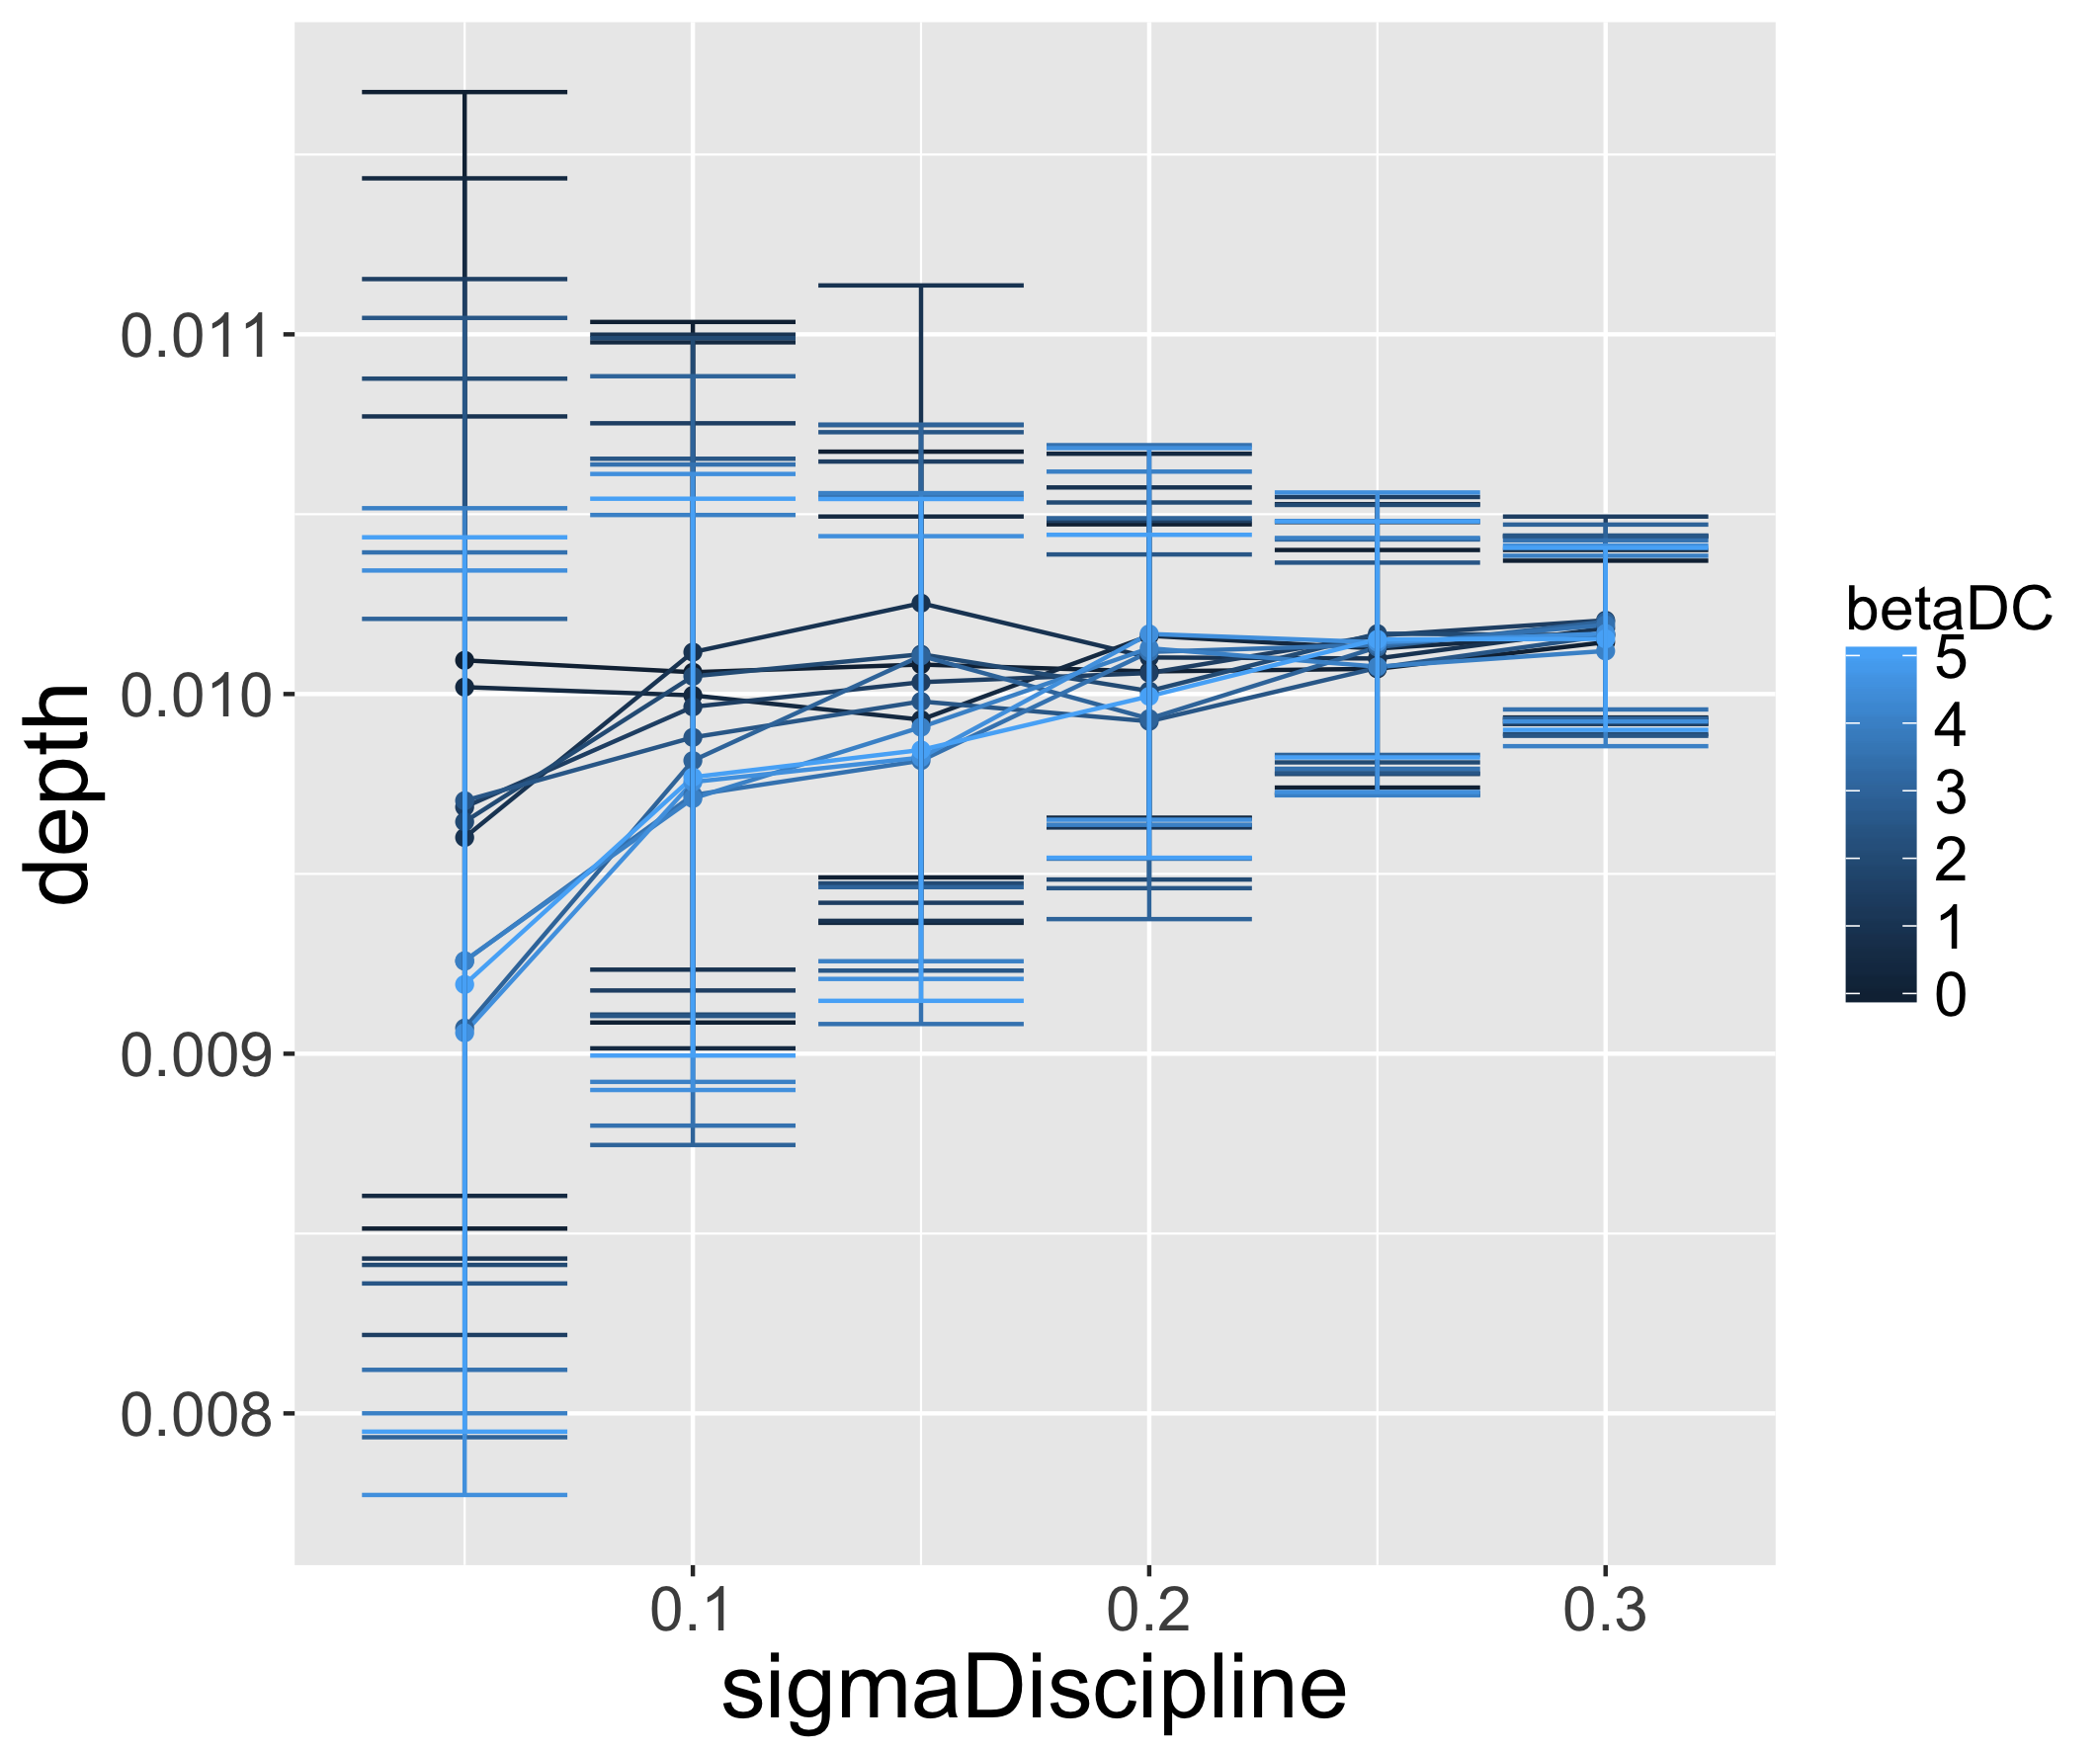
\includegraphics[width=0.32\linewidth]{figures/depth-sigma_alpha0-5_rho0}
%	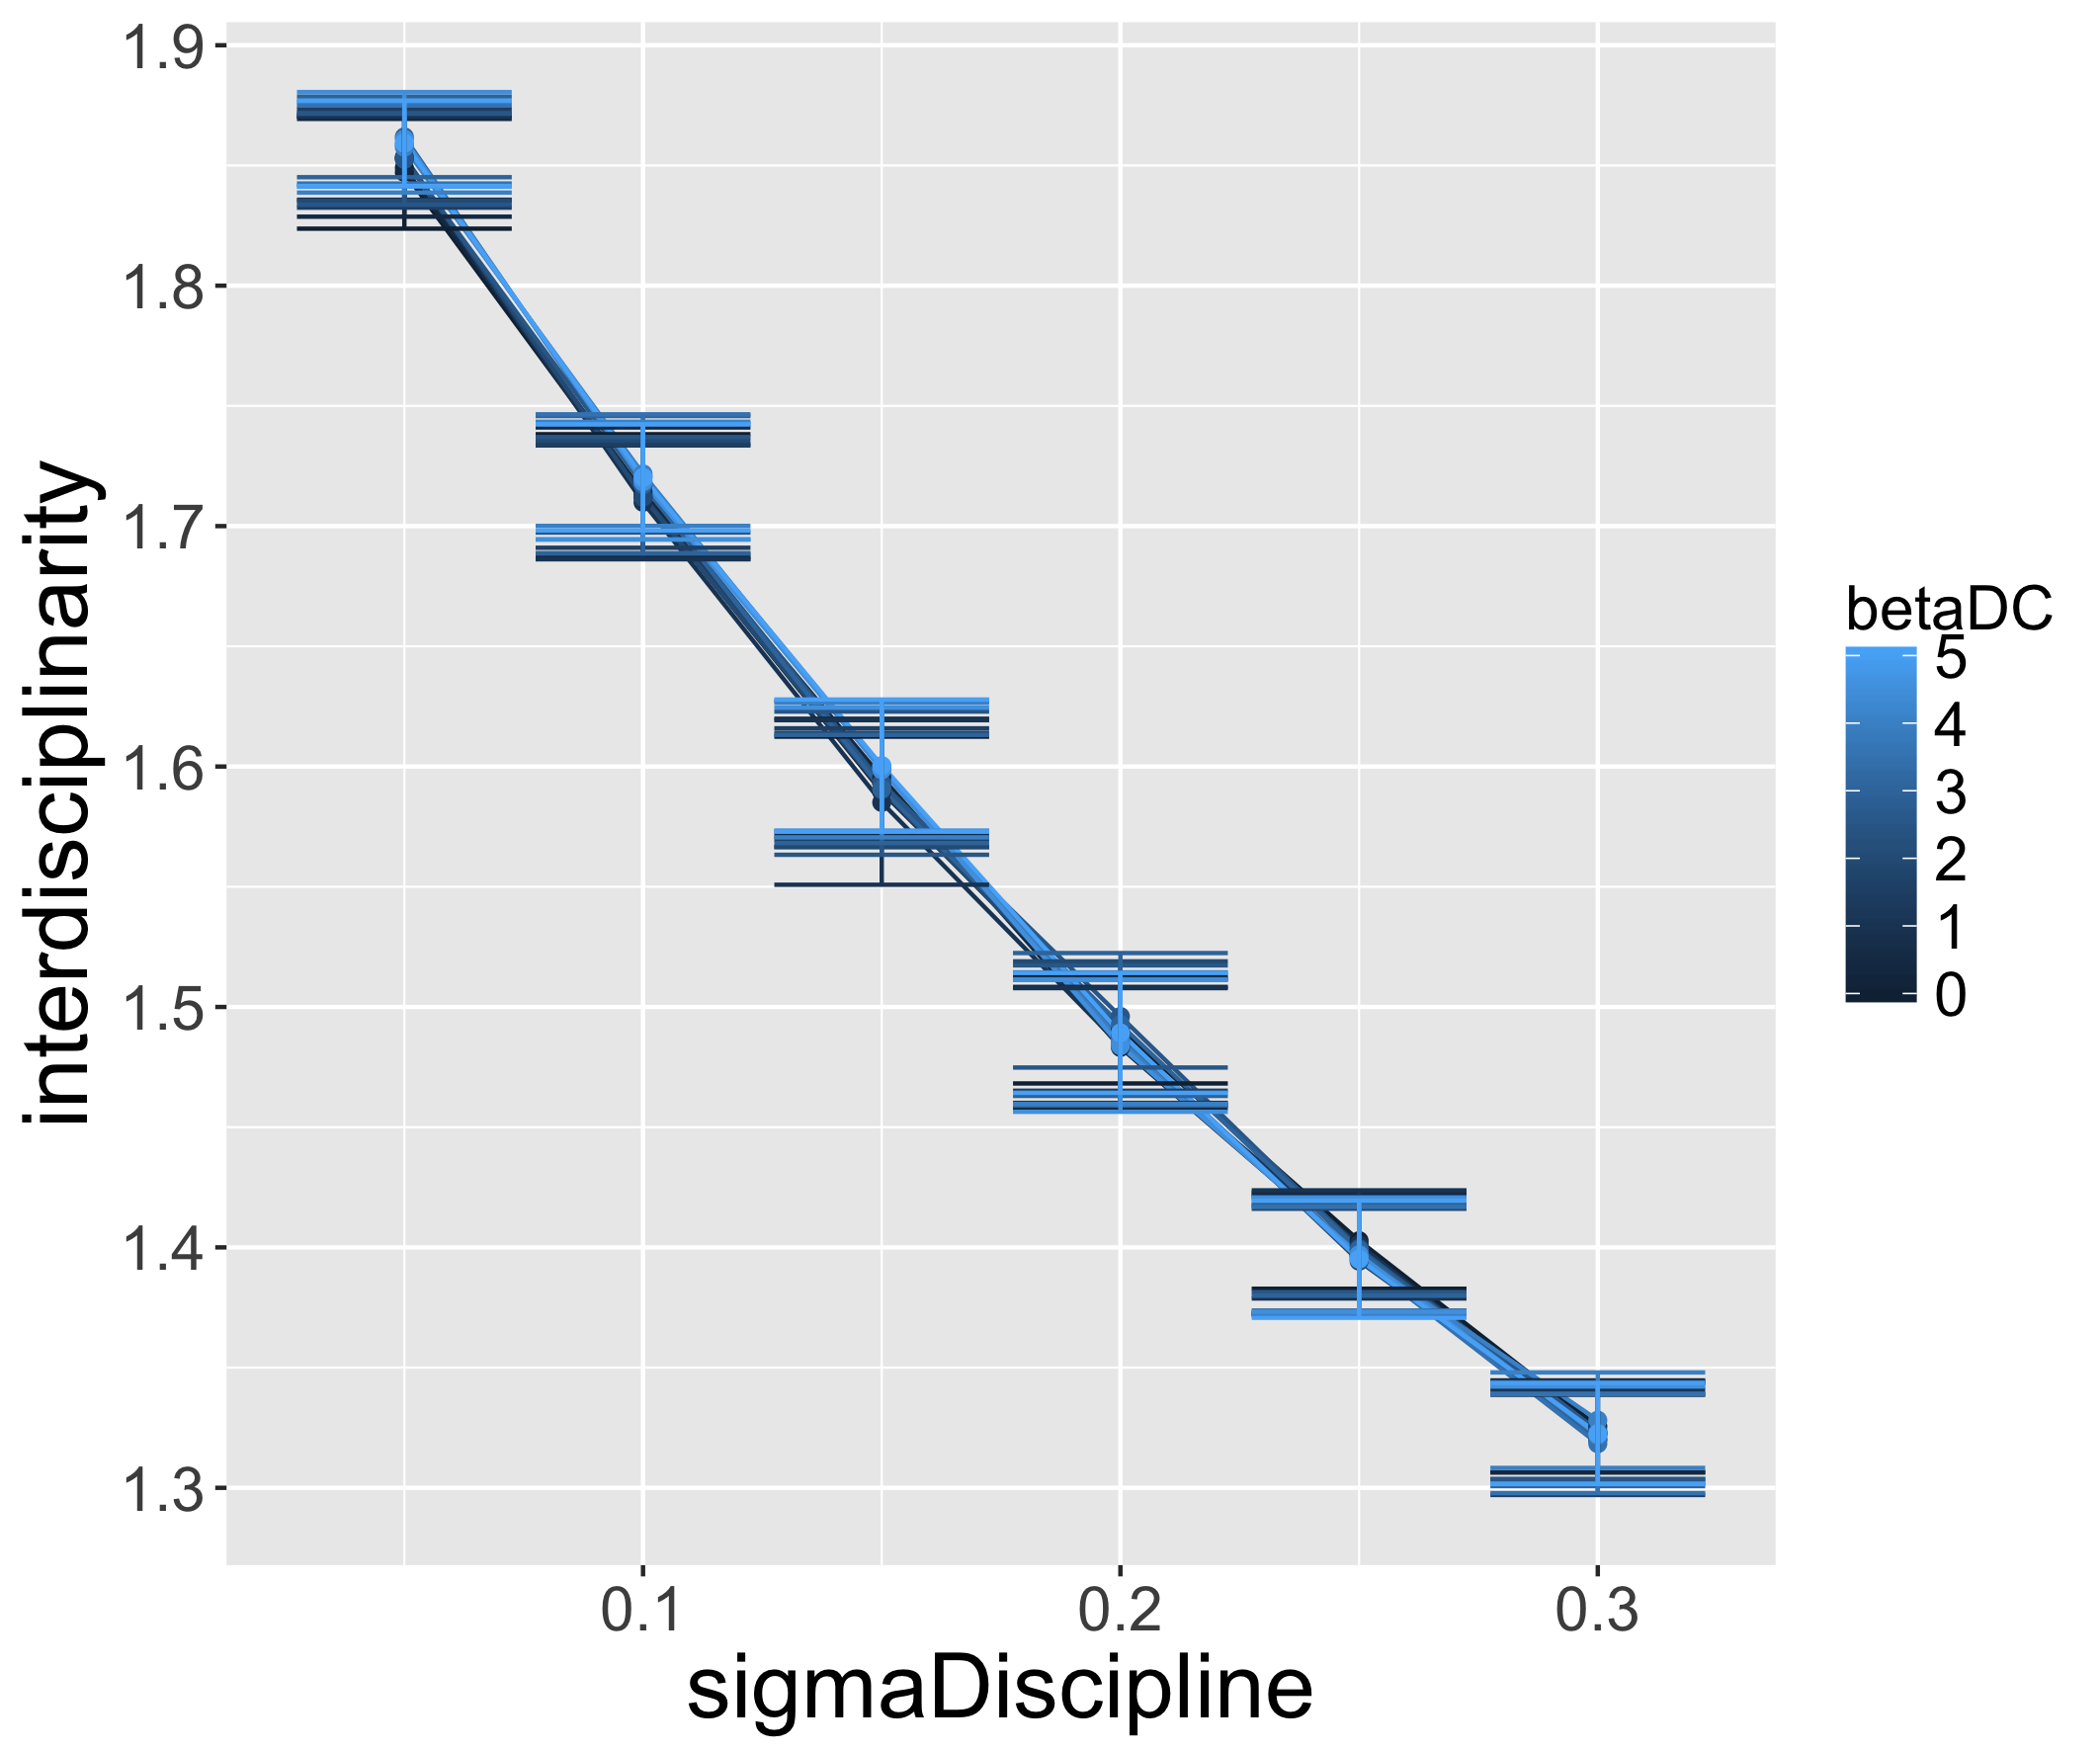
\includegraphics[width=0.32\linewidth]{figures/interdisc-sigma_alpha0-5_rho0}
%	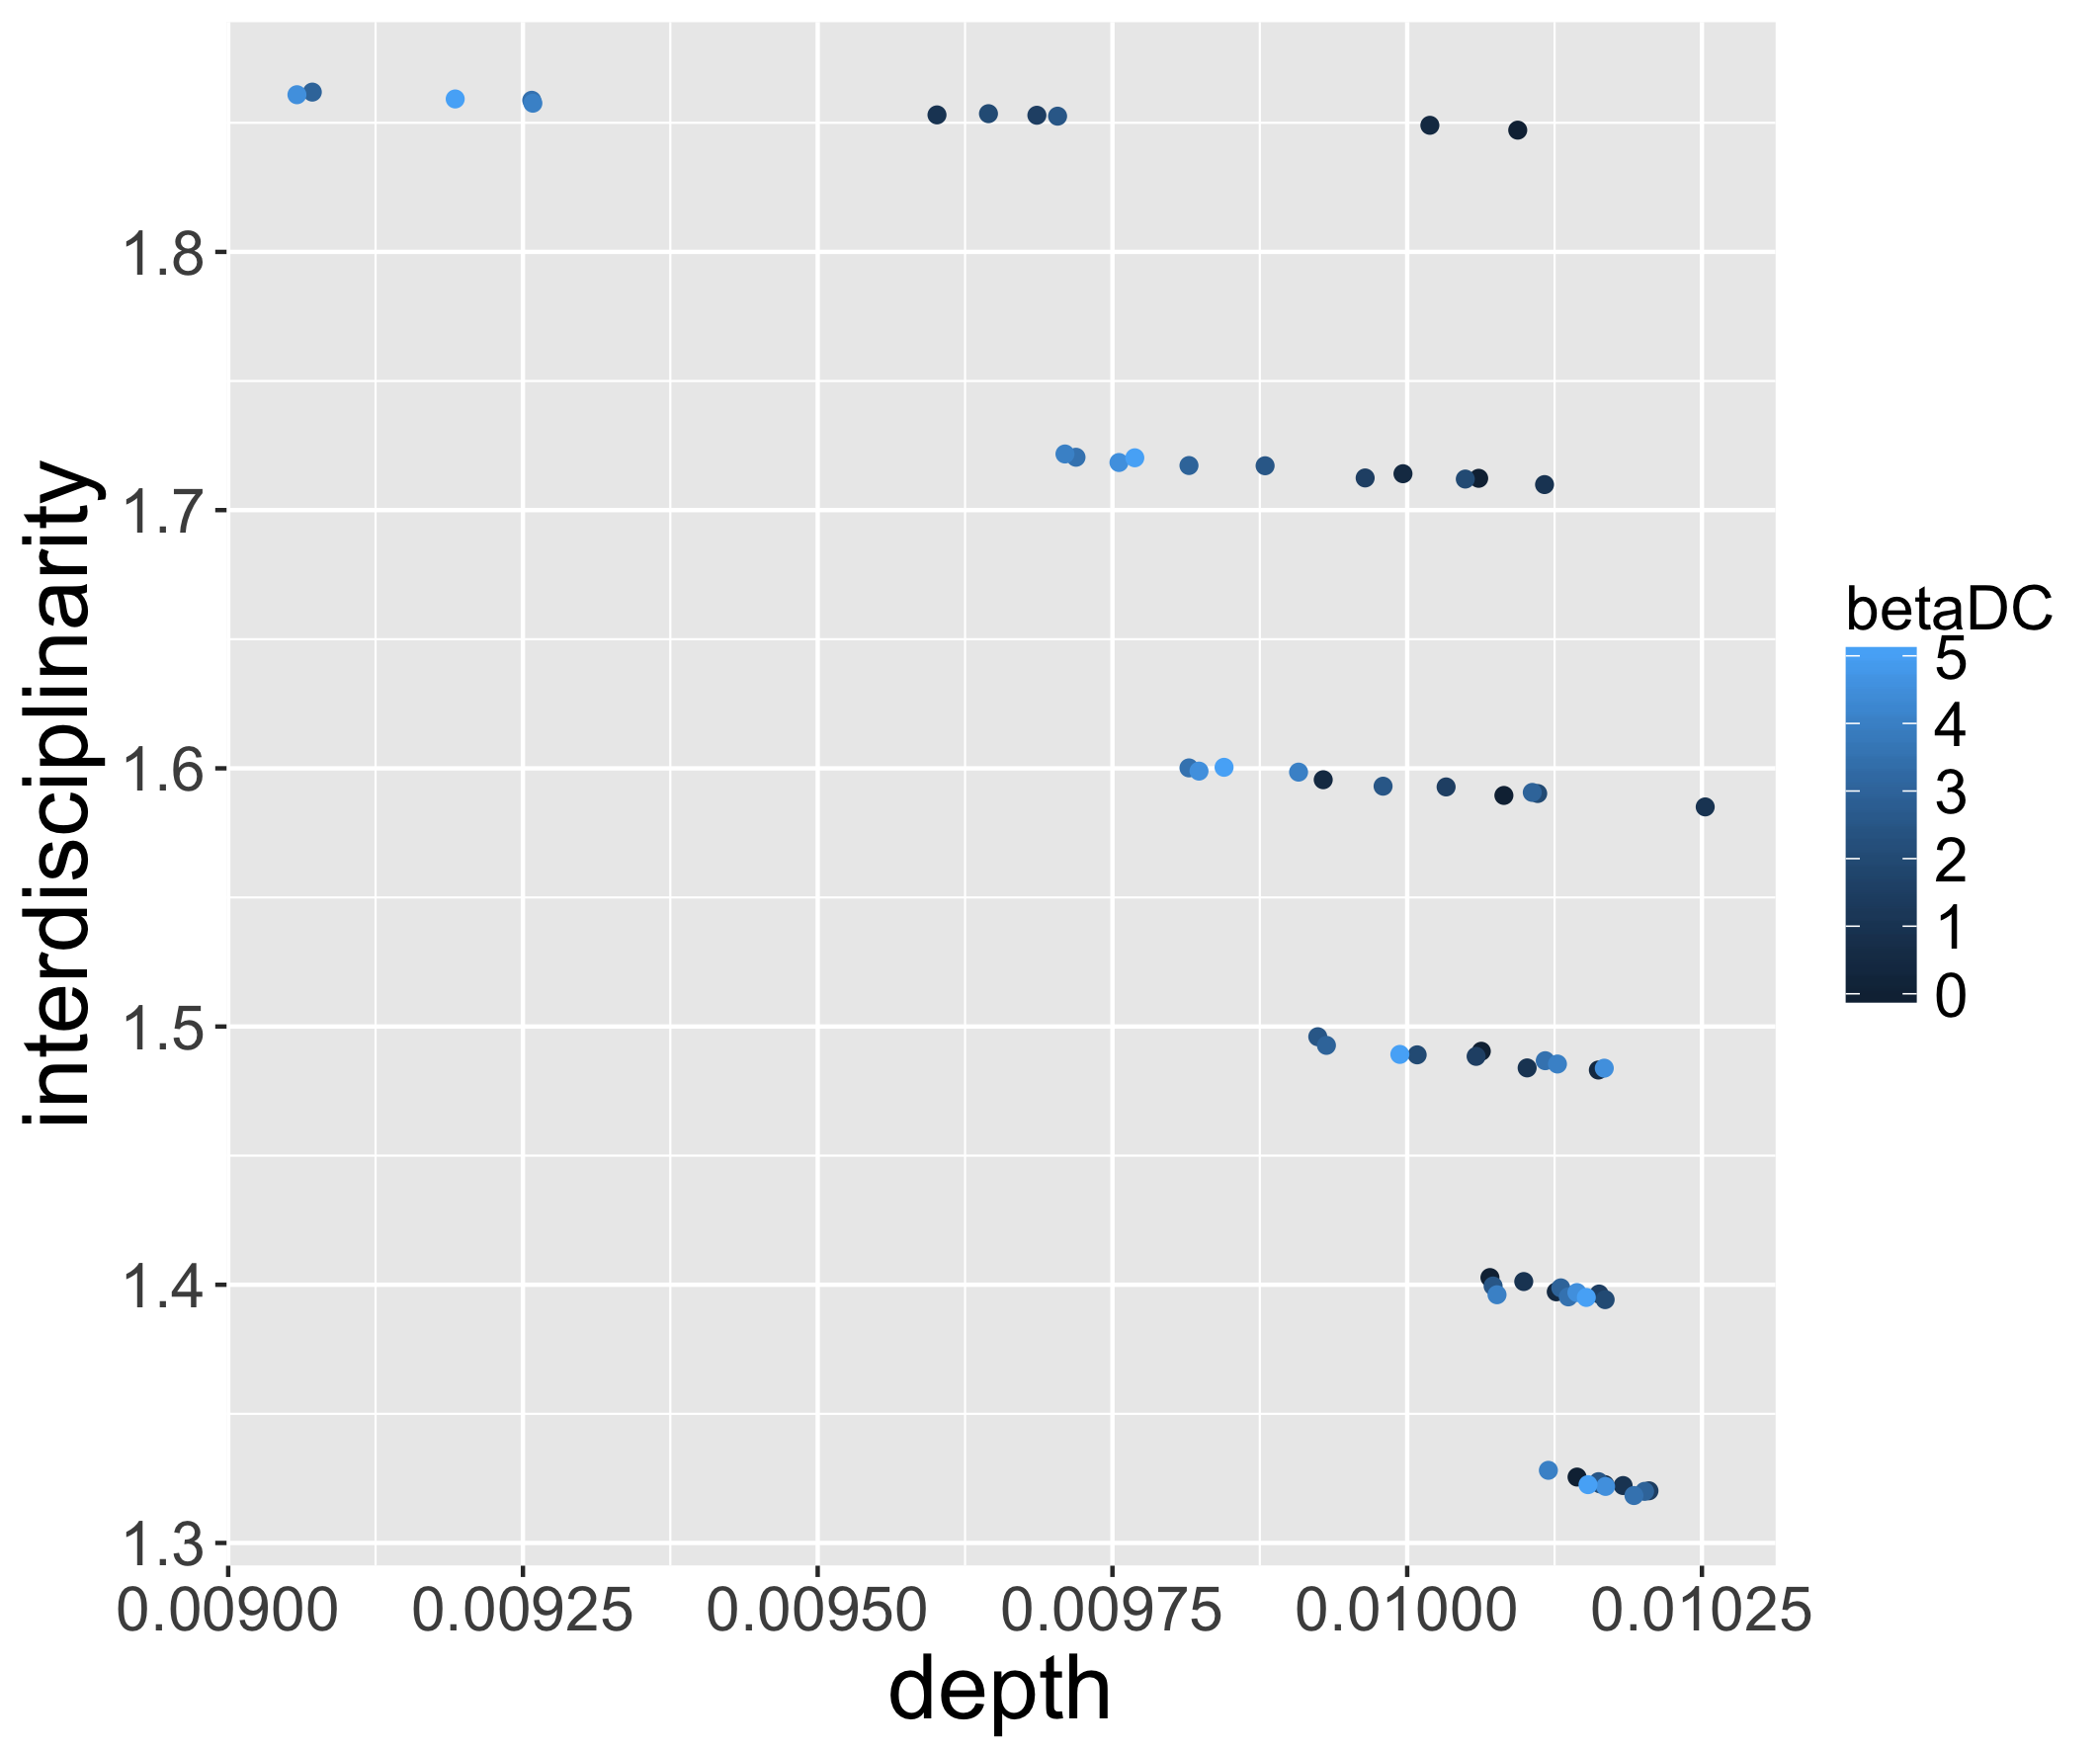
\includegraphics[width=0.32\linewidth]{figures/pareto_alpha0-5_rho0}
%	\caption{\textbf{Patterns of interdisciplinarity from model simulations.} We show measures of depth and interdisciplinarity (left and middle) at fixed $\alpha=0.5$ and network structure, for varying discrete choice parameter $\beta$ as a function of individual extent $\sigma$. On the right, the Pareto front of average point between these two objectives.}
%	\label{fig:plots}
%\end{figure*}
%


\end{document}
